\documentclass[frenchb, 11pt]{article}

\usepackage[top=2cm, bottom=2cm, left=2cm, right=2cm]{geometry}
\usepackage[utf8]{inputenc}
\usepackage[T1]{fontenc}
\usepackage{babel}

\usepackage{multicol}
\setlength{\columnseprule}{1pt} % separation line between columns

\usepackage{hyperref}
\hypersetup{
	colorlinks=true,	% false: boxed links; true: colored links
	linkcolor=black,	% color of internal links
	urlcolor=blue,		% color of external links
	citecolor=blue
}

\usepackage{graphicx}	% import graphics
\usepackage{wrapfig}	% wrap text around figures
\usepackage{subcaption}


\usepackage{verbatim}	% multi-line comments

% Colors
\usepackage[usenames,dvipsnames]{xcolor}

% Colored frame
\usepackage{framed}
\definecolor{shadecolor}{rgb}{0.96,0.96,0.96}
\definecolor{TFFrameColor}{rgb}{0.96,0.96,0.96}
\definecolor{TFTitleColor}{rgb}{0.00,0.00,0.00}

% Redefine leftbar envvironment
\newlength{\leftbarwidth}
\setlength{\leftbarwidth}{1pt}
\newlength{\leftbarsep}
\setlength{\leftbarsep}{10pt}

\newcommand*{\leftbarcolorcmd}{\color{leftbarcolor}} % as a command to be more flexible
\colorlet{leftbarcolor}{gray}

\renewenvironment{leftbar}{%
    \def\FrameCommand{{\leftbarcolorcmd{\vrule width \leftbarwidth\relax\hspace {\leftbarsep}}}}%
    \MakeFramed {\advance \hsize -\width \FrameRestore }%
}{%
    \endMakeFramed
}

% Code listings
\usepackage{listings}
\definecolor{dkgreen}{rgb}{0,0.6,0}
\definecolor{gray}{rgb}{0.5,0.5,0.5}
\definecolor{mauve}{rgb}{0.58,0,0.82}
\definecolor{blue}{rgb}{0,0,0.7}
\lstset{
	language=bash,
	basicstyle=\scriptsize,
	numbers=left,                   % where to put the line-numbers
  	numberstyle=\tiny\color{gray},
	commentstyle=\color{dkgreen},
	stringstyle=\color{BrickRed},
	backgroundcolor=\color{shadecolor},
    keywordstyle=\color{OliveGreen},
	frame=single,                   % adds a frame around the code
 	rulecolor=\color{black},
	emph={},
	emphstyle=\color{mauve},
	morekeywords={},
	keywordstyle={\color{black}},
	showstringspaces=false,
  	tabsize=4,
	moredelim=[is][\small\ttfamily]{/*}{*/}
}

% Title page
\title{
	\textbf{IT-3005 - TP Sécurité}\\
	DMZ / Firewall Linux
}
\date{\today}

\begin{document}
\maketitle
\newpage

%\tableofcontents
%\newpage

\section{Introduction}
% postes utilisés 10,11,12
% objectifs

\section{Câblage}
% TODO parler de mii-tool

\begin{figure}[h!]
	\centering
	\begin{subfigure}[b]{0.4\textwidth}
		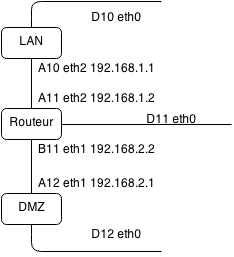
\includegraphics[scale=0.80]{sch1.png}
		\caption{Séance}
	\end{subfigure}%
	~
	\begin{subfigure}[b]{0.4\textwidth}
	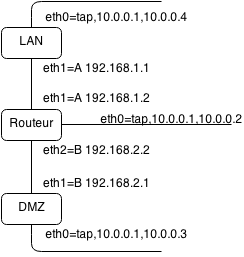
\includegraphics[scale=0.80]{sch2.png}
	\caption{Netkit}
	\label{fig:planadrnetkit}
	\end{subfigure}
	\caption{Plan d'adressage}
\end{figure}

\noindent \textbf{N.B.} Le rapport décrira les différentes étapes du TP en suivant le plan d'adressage de la figure \ref{fig:planadrnetkit} (Netkit).

% après câblage ping possibles: lan <-> routeur et dmz <-> routeur
% il faut activer le routage IP sur le routeur

\newpage

\section{Routage classique}
Nous avons tout d'abord configuré les interfaces Ethernet des 3 machines, ajouté les passerelles par défaut pour LAN et DMZ, et activé le routage IP (IP forwarding) pour le routeur. Le routage IP permet de prendre des décisions concernant le chemin qu'un paquet doit prendre entre les différents réseaux.\\
% TODO plus de détails ip forwarding

\noindent Configuration du routeur
% TODO coloration syntaxique
\begin{lstlisting}
/*Router:~#*/ echo "1" > /proc/sys/net/ipv4/ip_forward
/*Router:~#*/ ifconfig eth1 192.168.1.2 netmask 255.255.255.0 up
/*Router:~#*/ ifconfig eth2 192.168.2.2 netmask 255.255.255.0 up

/*Router:~#*/ ifconfig
eth0      Link encap:Ethernet  HWaddr 76:f5:98:50:22:50
          inet addr:10.0.0.2  Bcast:10.255.255.255  Mask:255.0.0.0
          ...

eth1      Link encap:Ethernet  HWaddr 7e:a1:77:92:58:e8
          inet addr:192.168.1.2  Bcast:192.168.1.255  Mask:255.255.255.0
          ...

eth2      Link encap:Ethernet  HWaddr 0e:bd:8c:c5:14:02
          inet addr:192.168.2.2  Bcast:192.168.2.255  Mask:255.255.255.0
          ...

/*Router:~#*/ route -n
Kernel IP routing table
Destination     Gateway         Genmask         Flags Metric Ref    Use Iface
192.168.2.0     0.0.0.0         255.255.255.0   U     0      0        0 eth2
192.168.1.0     0.0.0.0         255.255.255.0   U     0      0        0 eth1
10.0.0.0        0.0.0.0         255.0.0.0       U     0      0        0 eth0
0.0.0.0         10.0.0.1        0.0.0.0         UG    0      0        0 eth0
\end{lstlisting}
\hfill

\begin{leftbar}
\noindent % Q1. TODO Q1
%/proc/sys enable/disable kernel features
%/proc/sys/net adjust network configuration on running machine
%/proc/sys/net/ipv4
\end{leftbar}

\noindent Configuration du pc LAN
\begin{lstlisting}
/*LAN:~#*/ ifconfig eth0 down
/*LAN:~#*/ ifconfig eth1 192.168.1.1 netmask 255.255.255.0 up
/*LAN:~#*/ route add default gw 192.168.1.2 eth1

/*LAN:~#*/ ifconfig
eth1      Link encap:Ethernet  HWaddr 42:a7:57:d3:a5:1b
          inet addr:192.168.1.1  Bcast:192.168.1.255  Mask:255.255.255.0
          ...

/*LAN:~#*/ route
Kernel IP routing table
Destination     Gateway         Genmask         Flags Metric Ref    Use Iface
192.168.1.0     *               255.255.255.0   U     0      0        0 eth1
default         192.168.1.2     0.0.0.0         UG    0      0        0 eth1

/*LAN:~#*/ route -n
Kernel IP routing table
Destination     Gateway         Genmask         Flags Metric Ref    Use Iface
192.168.1.0     0.0.0.0         255.255.255.0   U     0      0        0 eth1
0.0.0.0         192.168.1.2     0.0.0.0         UG    0      0        0 eth1
\end{lstlisting}

La commande \emph{route -n} permet d'afficher la table de routage IP en remplaçant les noms d'hôtes (provenant par exemple du fichier /etc/hosts) par des adresses numériques. Le symbole * est remplacé par \emph{0.0.0.0}, ce qui désigne la route par défaut.
\newpage

\noindent Configuration du pc DMZ
\begin{lstlisting}
/*DMZ:~#*/ ifconfig eth0 down
/*DMZ:~#*/ ifconfig eth1 192.168.2.1 netmask 255.255.255.0 up
/*DMZ:~#*/ route add default gw 192.168.2.2 eth1

/*DMZ:~#*/ ifconfig
eth1      Link encap:Ethernet  HWaddr 86:e8:ec:bc:60:67
          inet addr:192.168.2.1  Bcast:192.168.2.255  Mask:255.255.255.0
          ...

/*DMZ:~#*/ route -n
Kernel IP routing table
Destination     Gateway         Genmask         Flags Metric Ref    Use Iface
192.168.2.0     0.0.0.0         255.255.255.0   U     0      0        0 eth1
0.0.0.0         192.168.2.2     0.0.0.0         UG    0      0        0 eth1
\end{lstlisting}

\begin{leftbar}
\noindent Q2 %TODO Q2
\end{leftbar}

Suite aux configurations effectuées précédemment, il est possible d'effectuer des pings entre les 3 machines.
% TODO listing

% TODO édition fichier httpd.conf séance VS Netkit
% TODO screenshot lynx LAN + start httpd DMZ + tcpdump routeur (side by side)
\newpage

% TODO bibliography
\begin{thebibliography}{5}
\end{thebibliography}

\end{document}
